
\ifx\isEmbedded\undefined

\documentclass[12pt]{report}
	
% FONT RELATED
%\usepackage{times} %Move to times font
\usepackage[labelfont=bf,textfont=it]{caption}
\usepackage[utf8]{inputenc}

% LINKS, PAGE OF CONTENT, REF AND CROSS-REF, HEADERS/FOOTERS
\usepackage[hidelinks]{hyperref}
\usepackage{fancyhdr}
\usepackage{acronym}

% FIGURES, GRAPHICS, TABLES
\usepackage{graphicx}
\usepackage{parskip}
%\usepackage{subfigure}
\usepackage{subfig}
\usepackage{wrapfig}
\usepackage{subfloat}

% COLOURS, TEXT AND FORMATTING
\usepackage{array}
\usepackage{color}
\usepackage{setspace}
\usepackage{longtable}
\usepackage{multirow}

% ADVANCED MATHS, PSEUDO-CODE
\usepackage{amsmath}
\usepackage{alltt}
\usepackage{amsfonts}

% BIBLIOGRAPHY
\usepackage[authoryear]{natbib}
\bibpunct{(}{)}{;}{a}{,}{,}

% USE IN DISSER:

\setlength\oddsidemargin{0.85cm}
\setlength\evensidemargin{0.85cm}

\setlength\textheight{21.0cm}
\setlength\textwidth{15.0cm}

% indent at each new paragrapg
\setlength\parindent{0.5cm}

\setlength\topmargin{-0.2in}
\renewcommand{\baselinestretch}{1.3}

%REPORT

%\setlength\oddsidemargin{1cm}
%\setlength\evensidemargin{0.3in}
%%\setlength\headsep{2.5in}
%
%\setlength\textheight{9.0in}
%\setlength\textwidth{5.5in}
%
%% indent at each new paragrapg
%\setlength\parindent{0.5cm}
%
%%\setlength{\parskip}{10.5ex}
%
%\setlength\topmargin{-0.2in}

%\newcommand{\HRule}{\rule{\linewidth}{0.5mm}}
\newcommand{\HRule}{\rule{\linewidth}{0.0mm}}

% Color definitions (RGB model)
\definecolor{ms-comment}{rgb}{0.1, 0.4, 0.1}
\definecolor{ms-question}{rgb}{0.4, 0.0, 0.0}
\definecolor{ms-new}{rgb}{0.2, 0.4, 0.8}


\graphicspath{{../img/}}
\begin{document}
%\maketitle
\fi

\chapter{Introduction}
\label{chap:intro}

Currently, the presence of crowds in visual pieces, let they be films or video games, has acquired a lot of relevance. Scenes with a crowded train station, big streets full of pedestrians, tons of animals in a flock, troops of robots, hordes of zombies or armies of warriors can be found very often in modern films and games.

In the past, not many films could afford this kind of resources in their scenes, since the only way of having more characters was actually including more characters in the cast. The use of extras highly increases the cost of a production, besides the requirement of a strict coordination and proper training in some situations. One of the reasons of the boom of big masses in films was the arrival of new technologies in computer graphics and artificial intelligence. Alongside with this, the generation and simulation of virtual crowds became a reality, saving money and time and making the use of crowds affordable to big and small studios.

Other of the reasons of the popularity of big groups of individuals featured in films is the strength they give to a shot. It is not only a matter of fact that crowds are visually stunning and their magnificence captures the attention of the audience, but also they are powerful tools to tell and enrich a story. At this point of time, it could be hard, if not impossible, to imagine the saga of the Lord of the Rings without those epic battles of tens of thousands of warriors, or imagine the breathtaking apocalyptic scenes without those milliards of zombies wandering around.

Closely tied to the idea of crowd simulation, the concept of behaviour appears. This is what gives life to the crowd and makes the spectator perceive the group nature of it. An army of brave warriors in a battlefield will find enemies and will show aggressive movements; on the other hand, on a ballroom gentlemen and ladies will dance graciously.

\begin{figure}[!h]
  \centering
  \begin{tabular}{c c}
  	\subfloat[Crowd in a train station]{\label{fig:f1}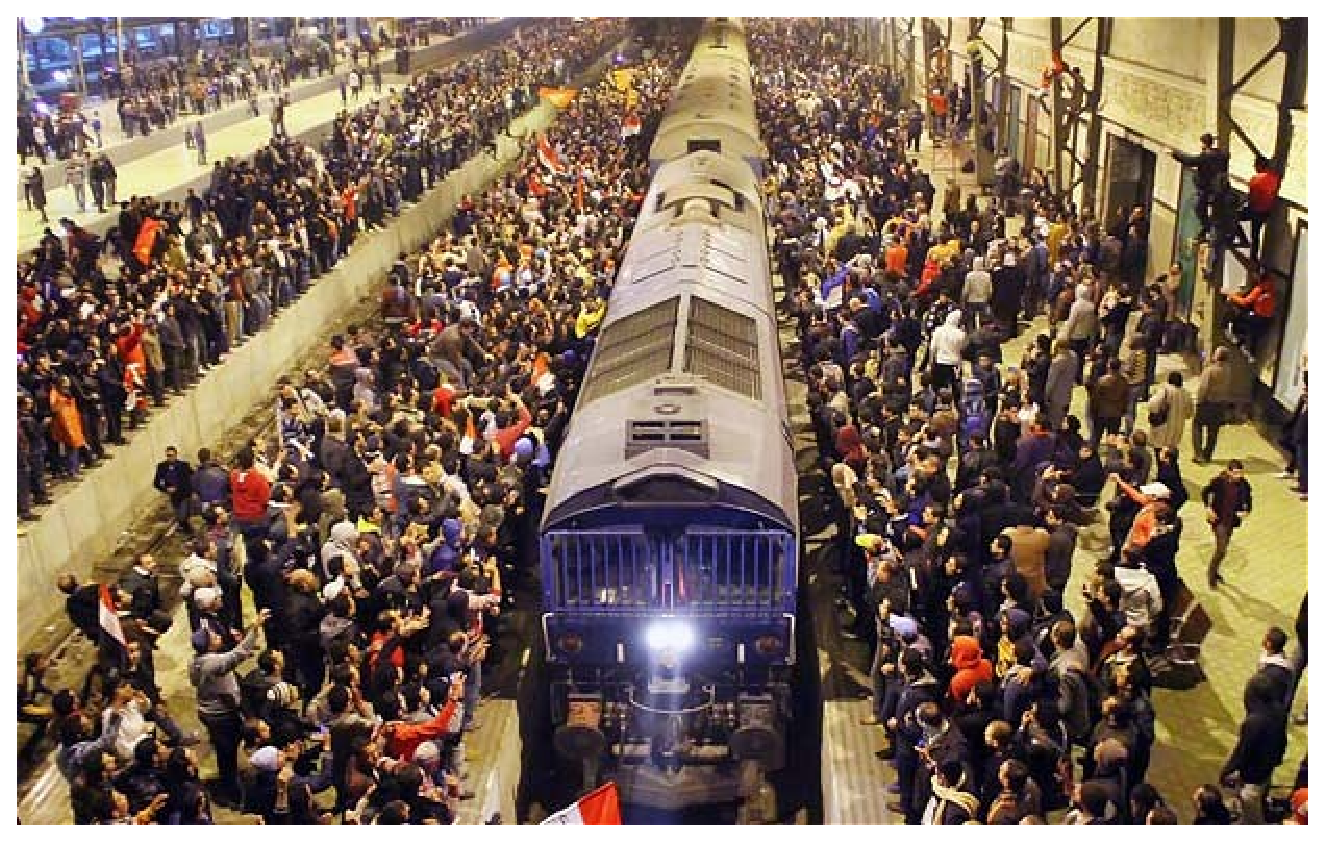
\includegraphics[scale=0.25]{crowd_train.eps}} &
 	\subfloat[Troops of droids (Star Wars)]{\label{fig:f2}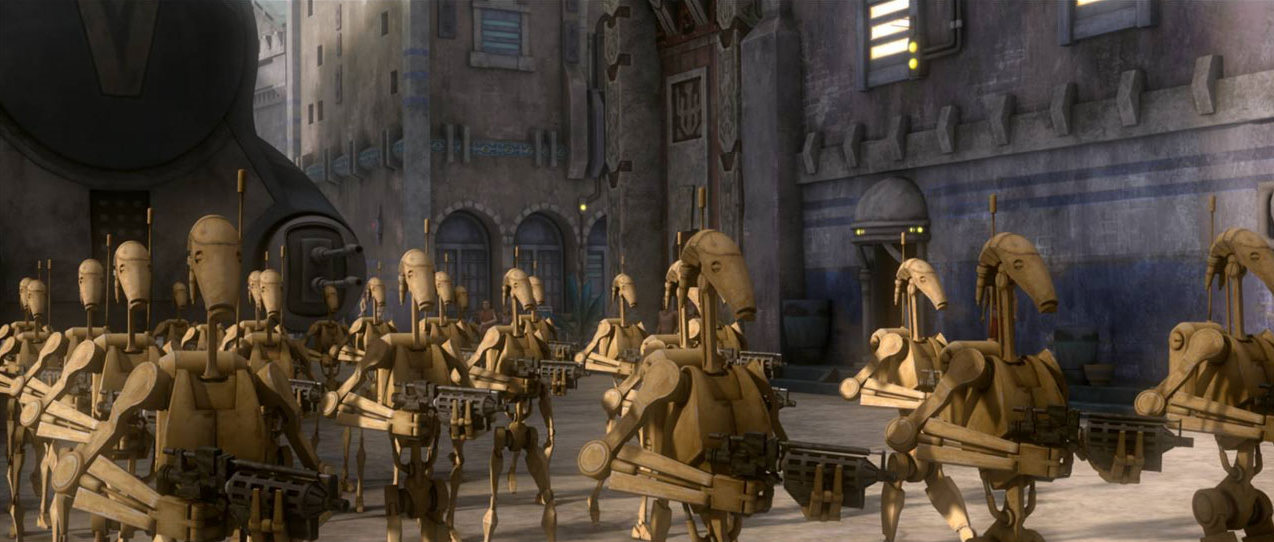
\includegraphics[scale=0.18]{droids.eps}} \\
  	\subfloat[Horde of zombies (World War Z)]{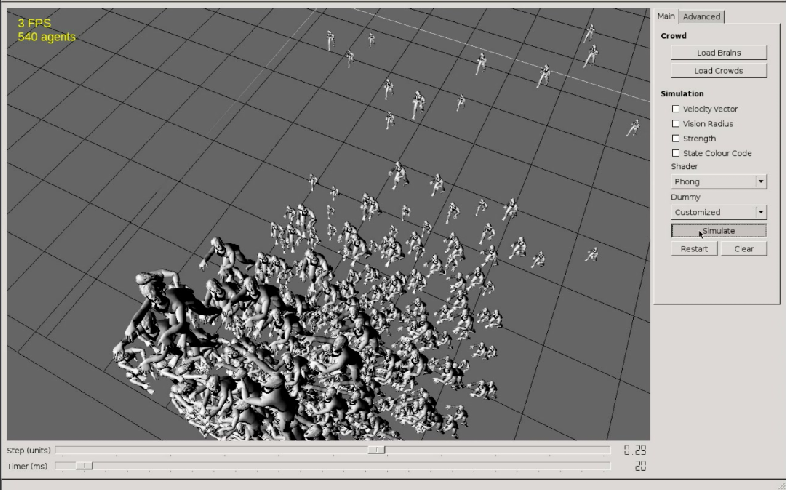
\includegraphics[scale=0.1]{zombies.eps}} & 
  	\subfloat[A Battlefield (Lord of the Rings))]{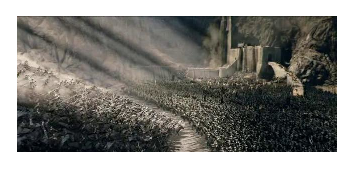
\includegraphics[scale=1.5]{battlefield.eps}} \\
  	\subfloat[A Ballroom]{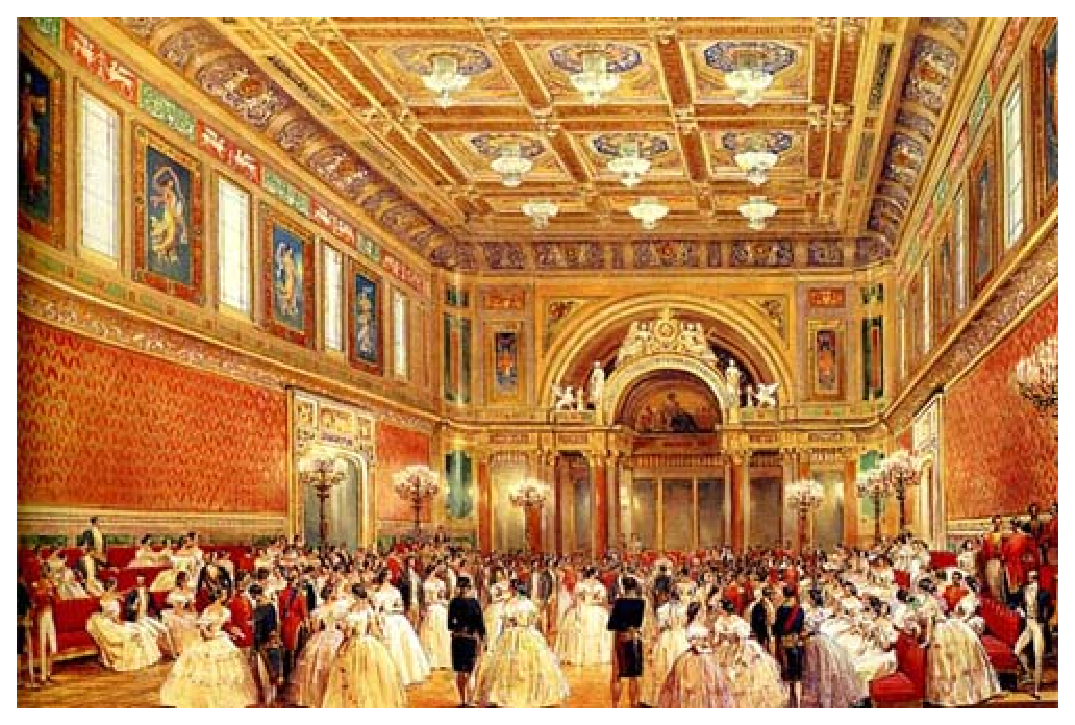
\includegraphics[scale=0.3]{ballroom.eps}} & 
  	\subfloat[One vs Many (Matrix)]{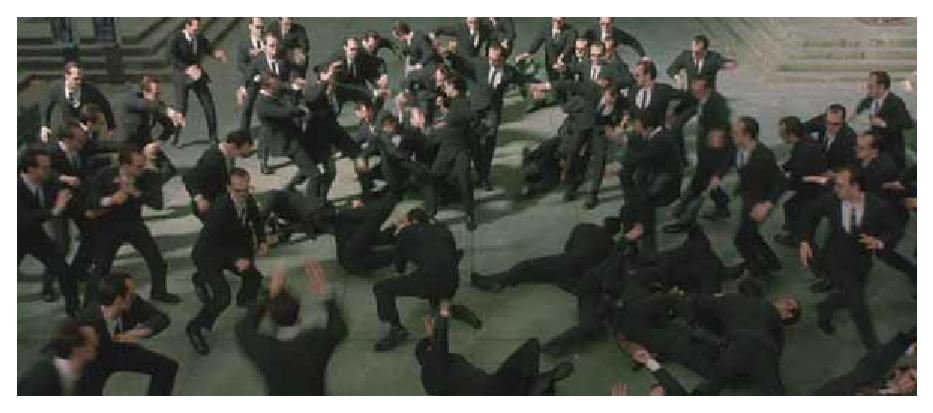
\includegraphics[scale=0.55]{matrix.eps}} \\
 \end{tabular}
  \caption{Crowd scenes}
  \label{fig:crowds}
\end{figure}

The aim of this project is to propose an approach which gives the flexibility to simulate any sort of crowd needed for a scene. Taking base on how the real world works, this method is based on the principle that the group behaviour is determined by the specific behaviours of every individual. And here is where one of the main ideas for this project appears: Emergent Behaviour.

Leonard Kleinrock, professor of computer science in UCLA, states that emergent behaviour is unanticipated behaviour shown by a system \citep{kleinrock}. Once a system is designed and defined by certain rules or mathematical equations, it may configure itself in a way that could not be anticipated. The interaction of a large number of simple individual things is very hard to predict; the complexity does not reside in the individuals, but on the way they are interconnected and they interact to each other. Professor Kleinrock proposes this example: ``we might know how a bunch of children behave when they are alone, but once you put them together in a group, you will observe behaviours that will surprise you''.

Subsequently, how a real crowd behaves is something hard to predict, and how realistic it is depends directly on how realistic each individual is.

This thesis is structured as follows:

\begin{itemize}

\item {{\bf Chapter 2: Related Work.} It explains the previous approaches in this field, the similarities and differences to the proposed method, as well as the advantages and drawbacks they present.}

\item {{\bf Chapter 3: Technical Background.} Physical concepts, flocking algorithms and the force-based virtual world model; and state machines and how they can be used to model behaviours.}

\item {{\bf Chapter 4: Agent Based Model.} This is where the current method starts to be explained into details, using a bottom-up approach. This chapter presents how agents are modeled, the parts which form them and their properties, as well as how they communicate to each other.}

\item{{\bf Chapter 5: Crowd Engine.} Here the core of the approach is introduced. It is explained how to handle the agents efficiently, how the virtual world is designed employing a physically-based approach, and how messages and collisions are faced.}

\item {{\bf Chapter 6: Applications and results.} A pipeline where this methodology might fit in a real production situation is presented. Some results of different tests will be shown in this chapter; a set of individual behaviours will be presented and the emergent behaviour observed will be explained and discussed.}

\item{{\bf Chapter 7: Application design and implementation.} The design and implementation for the application based on this approach are exposed.}

\item {{\bf Chapter 8: Conclusion.} A final concluding chapter will summarize the whole approach, mentioning the main advantages and drawbacks, as well as presenting potential lines for future work.}

\end{itemize}

\ifx\isEmbedded\undefined
% References
\addcontentsline{toc}{chapter}{References}
\bibliographystyle{../ref/harvard}
\bibliography{../ref/master}
\pagebreak
\end{document}
\fi

